\documentclass{beamer}

\usepackage[main=english,finnish]{babel}
\usepackage{cmbright}
\usepackage{fontspec}
\usepackage{booktabs}
\usepackage{hyperref}
\usepackage{graphicx}
\usepackage{pifont}
\usepackage{layout}

\newcommand{\cmark}{\ding{51}}%
\newcommand{\xmark}{\ding{55}}%

\hypersetup{pdfencoding=auto}

\newsavebox{\mysavebox}
\newlength{\myrest}

%\usepackage{polyglossia}
\setsansfont[Ligatures = TeX,
             BoldFont  = CMU Bright SemiBold,
             ItalicFont = CMU Bright Oblique,
            ]{CMU Bright Roman}
\setmainfont[Ligatures = TeX,
             BoldFont  = CMU Bright SemiBold,
             ItalicFont = CMU Bright Oblique,
            ]{CMU Bright Roman}
\setmonofont[Ligatures = TeX,
             BoldFont  = CMU Typewriter Text Bold,
             ItalicFont = CMU Typewriter Text Oblique,
            ]{CMU Typewriter Text}
\usetheme{Madrid}

\mode<presentation>
\setbeamercovered{transparent}
\setbeamertemplate{enumerate items}[default]
\setbeamertemplate{itemize items}[default]

\title[Finnish language text mining]{Extraction, exploration and exploitation of diverse Finnish language texts}
\subtitle{TIES445 Data Mining project}
\author[Robertson, Kanushin \& Qing]{Frankie Robertson\inst{1} \and Max Kanushin\inst{2} \and Li Qing\inst{3}}
\institute[JYU, LETI, SWUFE]{\inst{1} University of Jyväskylä \and%
                      \inst{2} Saint Petersburg State Electrotechnical University \and%
                      \inst{3} South Western University of Finance and Economics
                    }

\date{18th of April, 2016}

\titlegraphic{
  
\includegraphics[height=1.5cm]{jyu.pdf}
  \hspace{1cm}
  
\includegraphics[height=1.5cm]{leti_logo.png}
}

\begin{document}

\section{Title}
\begin{frame}
  \titlepage{}
\end{frame}

\section{Contents}
\begin{frame}
\frametitle{Contents}
\begin{enumerate}
  \item Orientation and aims\pause{}
  \item Extraction (scraping + preprocessing)\pause{}
  \item Exploration (mainly visualisation through dimension reduction)\pause{}
  \item Exploitation (obtain metrics which could be useful for presentation directly to an end-user or for use within a larger application)
\end{enumerate}

\end{frame}

\section{Orientation \& aims}
\begin{frame}
\frametitle{Orientation}

\begin{itemize}
  \item The Finnish language is used in different ways in different contexts.\pause{}

  \item For Finnish in particular there is a marked difference between spoken and
        written Finnish.\pause{}

  \item There are more complex grammatical features of Finnish which are used
        only rarely (in particular many inflections are used only rarely).\pause{}

  \item Wouldn't it be nice to be able to distinguish between written and
        spoken and between less and more complex Finnish?
\end{itemize}

\end{frame}

\begin{frame}
\frametitle{Aims}

\begin{itemize}
  \item Create a data set which characterises the range of these two dimensions
        of Finnish. \textit{(Extraction)} \cmark{}\pause{}

  \item Create features based on this data set and visualise them.
        \textit{(Exploration)} \cmark{}\pause{}

  \item Create a model which can attempt to characterise unseen data.
        \textit{(Exploitation)} \xmark{} -- still at the ideas stage
\end{itemize}

\end{frame}

\section{Extraction}

\begin{frame}
  \frametitle{Sources}
  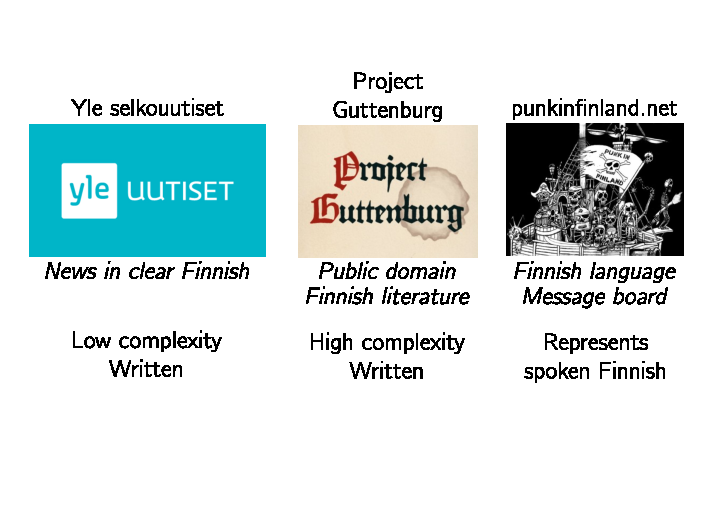
\includegraphics{sources.pdf}
\end{frame}

\begin{frame}
  \frametitle{Scraping \& data processing pipeline}
  \begin{columns}[onlytextwidth]
    \begin{column}{0.7\textwidth}
      \begin{itemize}
        \item We used Scrapy to write three custom spiders in Python. One key
          advantage of using Scrapy is that it makes it easy to write a reasonably
          well performing event based spider.\pause{}

        \item Another Python script converts the raw text into a series of
          matrices in a load'able .mat file using numpy \& scipy. The matrices
          are arranged in a similar way to the fisheriris data set.  Different
          features of the data are stored in different matrices...
      \end{itemize}
    \end{column}
      \begin{column}{0.3\textwidth}
      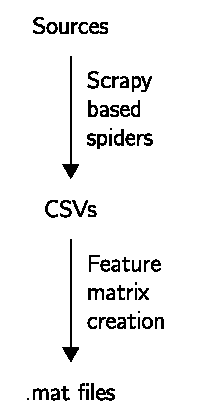
\includegraphics{pipeline.pdf}
    \end{column}
  \end{columns}
\end{frame}

\begin{frame}
  \frametitle{Preprocessing \& feature extraction}
  \begin{itemize}
    \item One set of matrices for distributions of word length and sentence
      length. Tokenisation using nltk.

    \item Other matrices based on gramatical analysis using FinnPos, a
      morphological analyser and part of speech tagger (built on top of another
      project called OMorFi).

    \item One matric measures inflection complexity. It should be possible to
      segment word forms into morphs (and get distribution of morphs per word)
      but requires in depth fiddling with FinnPOS. For the sake of time just
      used different between lemma length and word form length.

    \item Another set of matrices to represent part of speech distribution of
      individual words, pairs of words and and triplets of words (unigrams,
      bigrams, trigrams).
  \end{itemize}
\end{frame}

\begin{frame}
  \frametitle{Aside/soap box: the law}
  \begin{itemize}
    \item The legality of text mining on copyrighted material (which is pretty
      much everything recorded due to the Berne Convention) is unclear in the
      EU\pause{}

    \item In the US the recent Google Books case has cemented the the idea of a
      ``transformative factor'' of fair use (at least if you're Google)\pause{}

    \item Science Europe has published a detailed document about these issues:
      \href{http://www.scienceeurope.org/uploads/PublicDocumentsAndSpeeches/WGs_docs/SE_Briefing_Paper_textand_Data_web.pdf}%
      {Text and Data Mining and the Need for a Science-friendly EU Copyright Reform}\pause{}

    \item One of the recommendations is that research organisations should take a
      hands off approach and allow individual researchers to make their own
      choice as part of the process of pushing for new copyright exceptions
      rather than insisting on strict adherence to the obeying the letter of the
      law
  \end{itemize}
\end{frame}

\begin{frame}
  \frametitle{Exploration - dimension reduction on trigrams}
  \begin{columns}[t]
    \column{.5\textwidth}
      \centering
      \begin{figure}[H]
        \include[width=5cm,height=3.5cm]{lab1}\\
      \end{figure}
      \begin{figure}[H]
        \include[width=5cm,height=4cm]{lab2}
      \end{figure}
    \column{.5\textwidth}
      \centering
      \begin{figure}[H]
        \include[width=5cm,height=4cm]{lab3}\\
      \end{figure}
      \begin{figure}[H]
        \include[width=5cm,height=4cm]{lab4}
      \end{figure}
  \end{columns}
\end{frame}

\begin{frame}
  \frametitle{Ideas for exploitation}
  \begin{itemize}
    \item Original aim is to obtain a metric

    \item But this is an unsupervised situation (unless we make assumptions
      about the different sources as class labels) so simple regression is not
      possible

    \item If we can identify separate classes and characterise them with a
      metric, unseen data can be characterised by taking a weighted sum

    \item More sophisticated extensions might be possible, eg Guassian mixture
      models trained with expectation maximisation would consider different
      clusters to have different amounts of spread.
  \end{itemize}
\end{frame}

\begin{frame}
  \frametitle{Potential future work}
  \begin{itemize}
    \item Actually separate this data set.

    \item TD-IDF.

    \item Use segementation to enable a ``bag of morphs'' model. Useful
      since eg -ni, -si, -mme, -tte strongly suggest written language.

    \item Obtain a supervised data set.
  \end{itemize}
\end{frame}

\end{document}
